\documentclass[12pt,a4paper]{article}
\usepackage{graphicx}
\usepackage{geometry}
\usepackage{xcolor}
\usepackage{array}
\usepackage{longtable}
\usepackage{fancyhdr}
\usepackage{amsmath}
\geometry{margin=1in}
\usepackage{array}
\setlength{\headheight}{65pt}
\begin{document}
\noindent

\begin{center}
    \Large\textbf{\color{blue}Gate -PH 2011 46 Question}
\end{center}

\thispagestyle{fancy}
\fancyhf{}
\fancyhead[L]{
\includegraphics[height=2cm]{IIITB-COMET-Logo.png}}
\fancyhead[R]{ 
\begin{tabular}{r}
\textbf{Name:DARSI VAMSI} \\
\textbf{ID: COMETFWC071} \\
\end{tabular}
}
\section*{\color{blue}QUESTION}
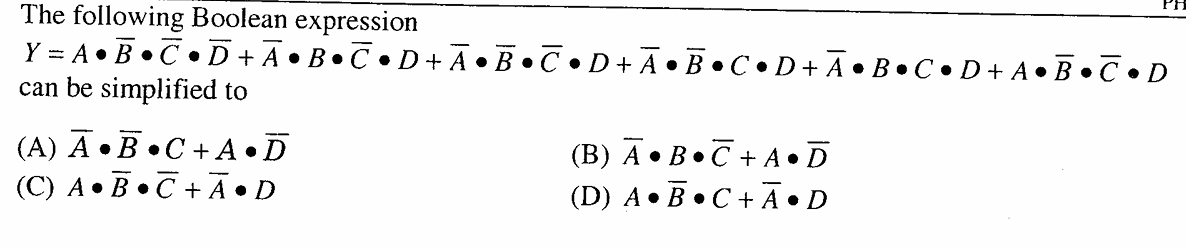
\includegraphics[width=1\textwidth,height=3cm]{PH 2011 46-esp32.png}
\section*{\color{blue}QUESTION ANALYSIS}
\section*{Solution}
can be simplified to

$$
\begin{array}{ll}
\textbf{(A)}\;
\overline{A}\cdot\overline{B}\cdot C
+
A\cdot\overline{D}
&
\textbf{(B)}\;
\overline{A}\cdot B\cdot\overline{C}
+
A\cdot\overline{D}
\\[0.5cm]
\textbf{(C)}\;
A\cdot\overline{B}\cdot\overline{C}
+
\overline{A}\cdot D
&
\textbf{(D)}\;
A\cdot\overline{B}\cdot C
+
\overline{A}\cdot D
\end{array}
$$

\section*{Solution}

Given,

$$
\begin{aligned}
Y=\;&
A\overline{B}\overline{C}\overline{D}
+\overline{A}B\overline{C}D
+\overline{A}\overline{B}\overline{C}D\\
&+\overline{A}\overline{B}CD
+\overline{A}BCD
+A\overline{B}\overline{C}D
\end{aligned}
$$

\subsection*{Step 1: Group the terms}

Group the first and last terms:

$$
A\overline{B}\overline{C}\overline{D}
+
A\overline{B}\overline{C}D
=
A\overline{B}\overline{C}
(\overline{D}+D)
$$

Since $\overline{D}+D=1$,

$$
A\overline{B}\overline{C}
(\overline{D}+D)
=
A\overline{B}\overline{C}.
$$

Now group the remaining four terms:

$$
\begin{aligned}
&
\overline{A}B\overline{C}D
+
\overline{A}\overline{B}\overline{C}D
+
\overline{A}\overline{B}CD
+
\overline{A}BCD
\\[0.2cm]
&=
\overline{A}D
\left(
B\overline{C}
+
\overline{B}\overline{C}
+
\overline{B}C
+
BC
\right).
\end{aligned}
$$

\subsection*{Step 2: Simplify inside the brackets}

$$
\begin{aligned}
&B\overline{C}
+\overline{B}\overline{C}
+\overline{B}C
+BC
\\[0.2cm]
&=
\overline{C}(B+\overline{B})
+
C(B+\overline{B})
\\[0.2cm]
&=
\overline{C}(1)
+
C(1)
\\[0.2cm]
&=
\overline{C}+C
\\[0.2cm]
&=1.
\end{aligned}
$$

Therefore,

$$
\overline{A}D(1)=\overline{A}D.
$$

\subsection*{Step 3: Final expression}

Hence,


$$
\boxed{
Y=
A\overline{B}\overline{C}
+
\overline{A}D
}
$$

This matches **Option (C).**

$$
\boxed{\text{Correct Answer: (C)}}
$$
\section*{Hardware Components Required}

\begin{table}[h]
\centering
\begin{tabular}{|c|l|}
\hline
\textbf{S.No.} & \textbf{Component} \\ \hline
1 & ESP32-WROOM Development Board \\ \hline
2 & Personal Computer (Ubuntu OS) \\ \hline
3 & USB Cable \\ \hline
4 & Breadboard \\ \hline
5 & 7447 BCD-to-7-Segment Decoder IC \\ \hline
6 & Common Anode 7-Segment Display \\ \hline
7 & 220 $\Omega$ Resistors (7 Nos.) \\ \hline
8 & Jumper Wires \\ \hline

\end{tabular}
\caption{Hardware and Software Components Required}
\label{tab:hardware}
\end{table}
\section*{Hardware Connections}

\begin{table}[h]
\centering
\begin{tabular}{|c|c|c|}
\hline
\textbf{S.No.} & \textbf{Connection} & \textbf{Description} \\ \hline
1 & ESP32 GPIO16 & 7447 Input A \\ \hline
2 & ESP32 GPIO17 & 7447 Input B \\ \hline
3 & ESP32 GPIO18 & 7447 Input C \\ \hline
4 & ESP32 GPIO19 & 7447 Input D \\ \hline
5 & ESP32 GND & 7447 GND \\ \hline
6 & ESP32 5V (VIN) & 7447 VCC \\ \hline
7 & 7447 Outputs (a--g) & 7-Segment Display Segments (a--g) \\ \hline
8 & Common Anode of 7-Segment & +5 V Supply \\ \hline
9 & Segment Lines & Through 220 $\Omega$ Resistors \\ \hline
10 & ESP32 USB Port & Ubuntu PC (Code Upload) \\ \hline
\end{tabular}
\caption{Hardware Connections for ESP32-WROOM with 7447 and Common Anode 7-Segment Display}
\label{tab:hardware_connections}
\end{table}
\section*{Execution Procedure}

\begin{enumerate}

\item Create a new PlatformIO project for the ESP32-WROOM board.

\begin{verbatim}
/root/venv/bin/pio project init --board esp32dev
\end{verbatim}

\item Place the source code (\texttt{main.cpp}) inside the \texttt{src} directory of the project.

\item Compile the source code and generate the binary files using:

\begin{verbatim}
/root/venv/bin/pio run
\end{verbatim}

\item After successful compilation, the following binary files are generated in the build directory:

\begin{verbatim}
.pio/build/esp32dev/
\end{verbatim}

\begin{itemize}
    \item \texttt{bootloader.bin}
    \item \texttt{partitions.bin}
    \item \texttt{firmware.bin}
\end{itemize}

\item Copy the generated binary files to the desired directory on the Ubuntu PC.

\item Connect the ESP32-WROOM board to the Ubuntu PC using a USB cable.

\item Verify that the ESP32 board is detected by the operating system.

\begin{verbatim}
ls -l /dev/ttyUSB*
\end{verbatim}

\item Verify the ESP32 chip.

\begin{verbatim}
esptool.py --chip esp32 --port /dev/ttyUSB0 chip_id
\end{verbatim}

\item Flash the generated binary files into the ESP32.

\begin{verbatim}
esptool.py --chip esp32 \
  --port /dev/ttyUSB0 \
  --baud 460800 \
  write_flash \
  0x1000 bootloader.bin \
  0x8000 partitions.bin \
  0x10000 firmware.bin
\end{verbatim}

\item Wait until the flashing process completes successfully.

\item Press the \textbf{EN (Reset)} button on the ESP32 board if required.

\item Observe the LED connected to the output GPIO pin to verify the implemented Boolean expression.

\end{enumerate}
\section*{Results and Observations}

The simplified Boolean expression,

$$
Y=A\overline{B}\,\overline{C}+\overline{A}D,
$$

was successfully implemented on the ESP32-WROOM development board. The output of the Boolean function was converted into BCD format and applied to the 7447 BCD-to-7-segment decoder IC. The decoder drove a common anode 7-segment display to indicate the output of the Boolean expression. The generated binary files were successfully flashed onto the ESP32, and the experimental output matched the expected truth table for all possible input combinations.

\subsection*{Truth Table}

\begin{table}[h]
\centering
\begin{tabular}{|c|c|c|c|c|c|}
\hline
A & B & C & D & $Y$ & 7-Segment Display \\ \hline
0 & 0 & 0 & 0 & 0 & 0 \\ \hline
0 & 0 & 0 & 1 & 1 & 1 \\ \hline
0 & 0 & 1 & 0 & 0 & 0 \\ \hline
0 & 0 & 1 & 1 & 1 & 1 \\ \hline
0 & 1 & 0 & 0 & 0 & 0 \\ \hline
0 & 1 & 0 & 1 & 1 & 1 \\ \hline
0 & 1 & 1 & 0 & 0 & 0 \\ \hline
0 & 1 & 1 & 1 & 1 & 1 \\ \hline
1 & 0 & 0 & 0 & 1 & 1 \\ \hline
1 & 0 & 0 & 1 & 1 & 1 \\ \hline
1 & 0 & 1 & 0 & 0 & 0 \\ \hline
1 & 0 & 1 & 1 & 0 & 0 \\ \hline
1 & 1 & 0 & 0 & 0 & 0 \\ \hline
1 & 1 & 0 & 1 & 0 & 0 \\ \hline
1 & 1 & 1 & 0 & 0 & 0 \\ \hline
1 & 1 & 1 & 1 & 0 & 0 \\ \hline
\end{tabular}
\caption{Truth Table of the Implemented Boolean Expression}
\label{tab:truth_table}
\end{table}

\subsection*{Experimental Output}

\begin{figure}[h]
\centering
% \includegraphics[width=0.45\textwidth]{seven_segment_0.jpg}
\caption{7-Segment Display showing digit '0' corresponding to Logic LOW ($Y=0$).}
\label{fig:display0}
\end{figure}

\begin{figure}[h]
\centering
% \includegraphics[width=0.45\textwidth]{seven_segment_1.jpg}
\caption{7-Segment Display showing digit '1' corresponding to Logic HIGH ($Y=1$).}
\label{fig:display1}
\end{figure}

\subsection*{Observation}

Figure~\ref{fig:display0} shows the 7-segment display indicating the digit '0' when the output of the Boolean expression is logic LOW ($Y=0$). Figure~\ref{fig:display1} shows the 7-segment display indicating the digit '1' when the output is logic HIGH ($Y=1$). The observed outputs were in agreement with the theoretical truth table.
\subsection*{Experimental Output}

\begin{figure}[h]
\centering
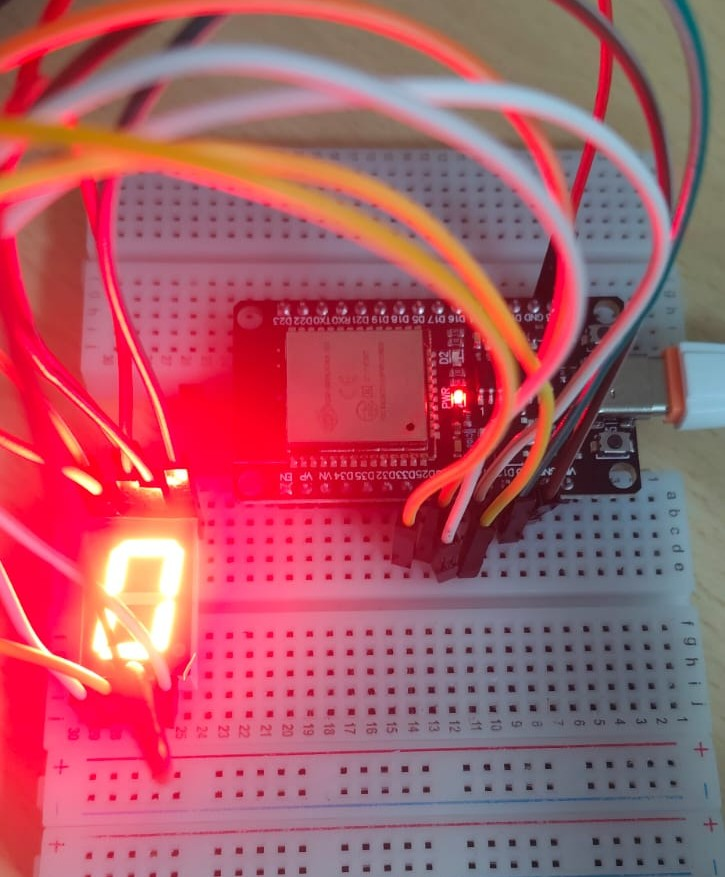
\includegraphics[width=0.45\textwidth]{7seg_0.jpeg}
\caption{7-Segment Display showing digit '0' corresponding to Logic LOW ($Y=0$).}
\label{fig:display0}
\end{figure}

\begin{figure}[h]
\centering
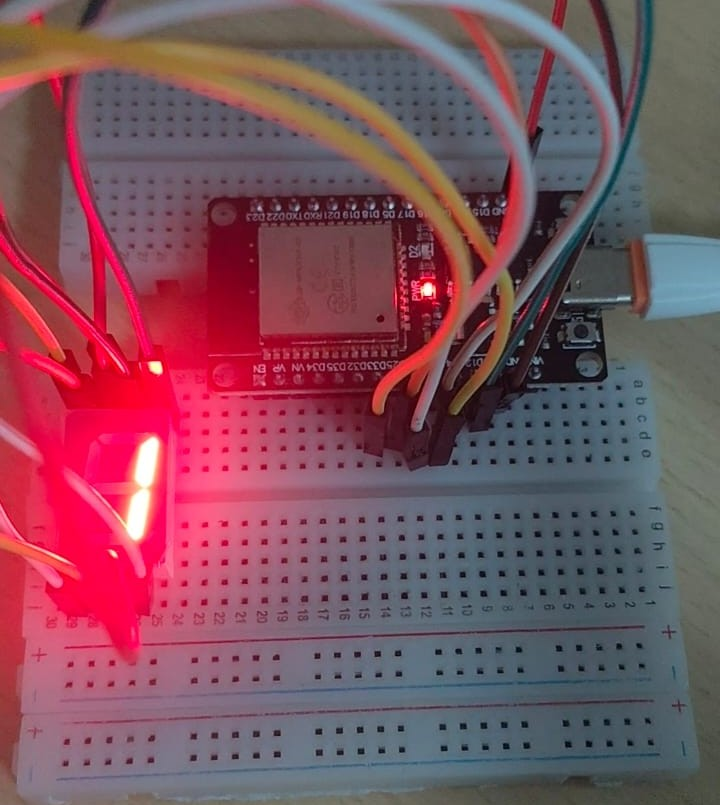
\includegraphics[width=0.45\textwidth]{7seg_1.jpeg}
\caption{7-Segment Display showing digit '1' corresponding to Logic HIGH ($Y=1$).}
\label{fig:display1}
\end{figure}

\subsection*{Result}

The Boolean expression was successfully implemented and verified using the ESP32-WROOM development board, 7447 BCD-to-7-segment decoder IC, and common anode 7-segment display. The experimental results matched the expected outputs for all input combinations.
\end{document}
